\documentclass[11pt,a4paper,twocolumn]{article}
\usepackage[utf8]{inputenc}
\usepackage[T1]{fontenc}
\usepackage{lmodern}
\usepackage{amsmath,amssymb,amsfonts,amsthm}
\usepackage{mathtools}
\usepackage{geometry}
\usepackage{booktabs}
\usepackage{array}
\usepackage{graphicx}
\usepackage{xcolor}
\usepackage{listings}
\usepackage{tikz}
\usetikzlibrary{arrows.meta, positioning}
\usepackage{hyperref}
\usepackage{fancyhdr}
\usepackage{titlesec}

\geometry{top=2.0cm, bottom=2.2cm, left=1.6cm, right=1.6cm, columnsep=0.7cm}

\definecolor{darkblue}{RGB}{15, 45, 95}
\definecolor{codebg}{RGB}{246, 248, 250}
\definecolor{codeframe}{RGB}{210, 215, 222}

\hypersetup{
    colorlinks=true,
    linkcolor=darkblue,
    urlcolor=darkblue,
    citecolor=darkblue
}

\lstset{
    backgroundcolor=\color{codebg},
    frame=single,
    rulecolor=\color{codeframe},
    basicstyle=\ttfamily\footnotesize,
    breaklines=true,
    captionpos=b,
    keepspaces=true,
    showspaces=false,
    showstringspaces=false,
    showtabs=false
}

\tikzset{
    meter/.style={
        draw,
        fill=codebg,
        minimum width=0.55cm,
        minimum height=0.46cm,
        inner sep=0pt,
        path picture={
            \draw[thin] ([yshift=-2pt]path picture bounding box.center) ++(-0.17cm, 0) arc (180:0:0.17cm);
            \draw[-{Latex[length=2.5pt]}, thin] ([yshift=-2pt]path picture bounding box.center) -- ++(0.12cm, 0.21cm);
        }
    },
    bigmeter/.style={
        draw,
        fill=codebg,
        minimum width=0.70cm,
        minimum height=0.54cm,
        inner sep=0pt,
        path picture={
            \draw[thin] ([yshift=-2pt]path picture bounding box.center) ++(-0.22cm, 0) arc (180:0:0.22cm);
            \draw[-{Latex[length=2.5pt]}, thin] ([yshift=-2pt]path picture bounding box.center) -- ++(0.14cm, 0.25cm);
        }
    },
    gate/.style={
        draw,
        fill=white,
        minimum size=0.45cm,
        inner sep=1pt,
        font=\small
    },
    smallgate/.style={
        draw,
        fill=white,
        minimum width=0.39cm,
        minimum height=0.46cm,
        inner sep=0pt,
        font=\scriptsize
    },
    target/.style={
        circle,
        draw,
        inner sep=0pt,
        minimum size=3.5mm,
        path picture={
            \draw[thin] (path picture bounding box.north) -- (path picture bounding box.south)
                        (path picture bounding box.west) -- (path picture bounding box.east);
        }
    },
    control/.style={
        circle,
        fill=black,
        inner sep=0pt,
        minimum size=1.8mm
    }
}
\pagestyle{fancy}
\fancyhf{}
\fancyhead[L]{\footnotesize |BF> (Bra-Ket-Fuck): The Dirac--M\"uller Quantum Tape Architecture}
\fancyhead[R]{\footnotesize Technical Whitepaper $\cdot$ October 2026}
\fancyfoot[C]{\footnotesize \thepage}

\newcommand{\bra}[1]{\langle #1 |}
\newcommand{\ket}[1]{| #1 \rangle}
\newcommand{\braket}[2]{\langle #1 | #2 \rangle}
\newcommand{\ketbra}[2]{| #1 \rangle\langle #2 |}
\newtheorem{theorem}{Theorem}

\title{\vspace{-0.5cm}\textbf{\Large \texttt{|BF>} (Bra-Ket-Fuck): A Vacuum-Initialized Clifford+\ensuremath{T} Quantum Tape\protect\\ Architecture for Linear Nearest-Neighbor Compilation and Formal\protect\\ Verification}}
\author{\large mat-ocl (\href{https://github.com/mat-ocl}{\texttt{github.com/mat-ocl}})\\[3pt]
\normalsize Systems \& Quantum Esoteric Architecture Working Group\\[2pt]
\small Technical Whitepaper $\cdot$ Architecture Specification v1.0 $\cdot$ October 2026}
\date{}

\begin{document}

\twocolumn[
  \begin{@twocolumnfalse}
    \maketitle
    \begin{abstract}
      \noindent Modern quantum programming frameworks operate predominantly on high-level Directed Acyclic Graphs (DAGs) representing arbitrary all-to-all quantum circuits. While ergonomic for algorithm design, these abstractions obscure physical Linear Nearest-Neighbor (LNN) hardware constraints \cite{fowler2004lnn,saeedi2011lnn}, complicate formal verification in theorem provers \cite{rand2018voqc}, and leave quantum loop semantics ambiguous. Conversely, existing minimal esoteric quantum languages---most notably Ihope127's \emph{Quantum brainfuck} (QBF) \cite{ihope2006qbf}---suffer from non-physical $\ket{1}^{\otimes N}$ initialization, the absence of native Pauli bit-flip primitives, and exorbitant gate synthesis overhead. In this whitepaper, we introduce \textbf{\texttt{|BF>} (Bra-Ket-Fuck)} and its underlying execution model, the \textbf{Dirac--M\"uller Abstract Machine (DMM)}. \texttt{|BF>} unifies Urban M\"uller's minimal 1D tape pointer semantics \cite{muller1993brainfuck} with Paul Dirac's bra-ket Hilbert space formalism \cite{dirac1939notation,nielsen2010quantum} over a physical $\ket{0}^{\otimes N}$ vacuum ground state. We present the complete operational semantics of \texttt{|BF>}, prove its BQP-universality via the Clifford+$T$ universal basis \cite{boykin1999optimal,bravyi2005universal}, demonstrate its $8\times$ instruction-count reduction over QBF for the nearest-neighbor CNOT primitive, and specify an $O(1)$ per-instruction transpiler targeting \textbf{OpenQASM 3.0} \cite{cross2022openqasm3} dynamic circuits.
    \end{abstract}
    \vspace{0.6cm}
  \end{@twocolumnfalse}
]

\section{Introduction \& Motivation}

In classical theoretical computer science, Urban M\"uller's Brainfuck (1993) \cite{muller1993brainfuck} established an enduring milestone: demonstrating that a discrete tape machine requires only eight syntactic tokens (\texttt{> < + - . , [ ]}) to achieve Turing completeness. Far from being a mere curiosity, minimal instruction set architectures (ISAs) serve as foundational razors for compiler verification, decidability bounds, and hardware micro-architectures.

As quantum computing transitions from theoretical algorithms to Noisy Intermediate-Scale Quantum (NISQ) processors \cite{preskill2018nisq} and early fault-tolerant lattices, quantum software engineering faces an analogous foundational gap:
\begin{enumerate}
    \item \textbf{The QTM-to-Circuit Disconnect:} Bernstein and Vazirani (1993, 1997) \cite{bernstein1997quantum} formalized BQP (Bounded-Error Quantum Polynomial-Time) using Quantum Turing Machines (QTMs) with local tape heads. However, industrial languages (Qiskit, Cirq, OpenQASM \cite{cross2022openqasm3}, Q\#) abandon tape semantics for circuit DAGs that assume arbitrary non-local qubit connectivity.
    \item \textbf{Intractability of Formal Verification:} Proving the mathematical soundness of optimizing quantum compilers in proof assistants (Lean 4, Coq, Isabelle) is virtually impossible when the source language embeds full Python or complex type systems. A minimal 12-token BQP-universal calculus makes mechanized correctness proofs (in the spirit of the verified optimizer VOQC \cite{rand2018voqc}) tractable.
    \item \textbf{Dynamic Control Flow \& Halting:} Defining iteration (\texttt{[ ]}) when loop conditions reside in quantum superposition exposes fundamental tensions between unitary evolution and projective measurement (the quantum halting problem \cite{ozawa1998halting,linden1998halting}).
    \item \textbf{Compiler Fuzzing:} Optimizing transpilers rely on peephole synthesis and unitary equivalence checking ($U_{\text{opt}}^\dagger U_{\text{spec}} \propto I$). Minimal tape programs generate dense, non-idiomatic gate sequences ideal for differential fuzzing of industrial transpilers; the reference toolchain applies exactly this technique to itself, comparing the abstract machine, two independent transpiler implementations, and an exact OpenQASM interpreter on randomly generated programs.
\end{enumerate}

To address these challenges, we define \textbf{|BF> (Bra-Ket-Fuck)}---a play on Dirac's bra-ket notation ($\langle\psi||\phi\rangle$) \cite{dirac1939notation} and Brainfuck's pointer tokens (\texttt{<}, \texttt{>}).

\section{The Dirac--M\"uller Abstract Machine}

\subsection{State Space Formulation}
Let a \texttt{|BF>} machine of register width $N \in \mathbb{N}^+$ be defined as a tuple $\mathcal{M} = (\mathcal{H}_N, p, \mathcal{C})$, where:
\begin{itemize}
    \item $\mathcal{H}_N = (\mathbb{C}^2)^{\otimes N}$ is a $2^N$-dimensional complex Hilbert space spanned by the computational basis $\{\ket{b_0 b_1 \dots b_{N-1}} : b_k \in \{0,1\}\}$.
    \item The quantum tape initializes to the physical vacuum ground state:
    \begin{equation}
        \ket{\Psi_0} = \bigotimes_{k=0}^{N-1} \ket{0}_k = \ket{00\dots 0}
    \end{equation}
    \item $p \in \mathbb{Z}_N = \{0, 1, \dots, N-1\}$ is the classical tape head pointer initialized to $p_0 = 0$.
    \item $\mathcal{C} \in \{0,1\}^*$ is the classical measurement transcript stream.
\end{itemize}

At any execution step $t$, the composite state of the quantum register is represented by the normalized state vector:
\begin{equation}
\begin{aligned}
    \ket{\Psi(t)} &= \sum_{x=0}^{2^N - 1} \alpha_x(t) \ket{x}, \quad \alpha_x(t) \in \mathbb{C}, \\
    \sum_{x=0}^{2^N - 1} |\alpha_x(t)|^2 &= 1
\end{aligned}
\end{equation}

\subsection{Unitary Gate Primitives \& Hilbert Lifting}
Single-qubit instructions in \texttt{|BF>} act exclusively on the active cell $p$. To apply a local $2 \times 2$ unitary operator $G \in U(2)$ to qubit $p$, the machine constructs the lifted $2^N \times 2^N$ unitary operator $\mathcal{U}_p(G)$ via Kronecker tensor products:
\begin{equation}
    \mathcal{U}_p(G) = \left( \bigotimes_{k=0}^{p-1} I_2 \right) \otimes G \otimes \left( \bigotimes_{k=p+1}^{N-1} I_2 \right)
\end{equation}

The fundamental single-qubit gates mapped to \texttt{|BF>} tokens are:
\begin{equation}
    X_{\text{(+)}} = \begin{pmatrix} 0 & 1 \\ 1 & 0 \end{pmatrix}, \quad
    Z_{\text{(Z)}} = \begin{pmatrix} 1 & 0 \\ 0 & -1 \end{pmatrix}
\end{equation}
\begin{equation}
    H_{\text{(H)}} = \frac{1}{\sqrt{2}}\begin{pmatrix} 1 & 1 \\ 1 & -1 \end{pmatrix}, \quad
    T_{\text{(T)}} = \begin{pmatrix} 1 & 0 \\ 0 & e^{i\pi/4} \end{pmatrix}
\end{equation}
For exact reversibility, the decrement token \texttt{-} maps to the Hermitian adjoint of the phase shift $T^\dagger = \text{diag}(1, e^{-i\pi/4})$. Together with CNOT, the gate set $\{H, T, \text{CNOT}\}$ forms the Clifford+$T$ universal basis \cite{boykin1999optimal,bravyi2005universal}.

\subsection{Nearest-Neighbor Entanglement (\texttt{\^{}})}
To enforce physical Linear Nearest-Neighbor (LNN) locality \cite{fowler2004lnn,saeedi2011lnn}, \texttt{|BF>} restricts two-qubit interactions to adjacent cells $(p, p+1)$. The entanglement token \texttt{\^{}} applies a Controlled-NOT ($\text{CNOT}_{p \to p+1}$) with control qubit $p$ and target qubit $p+1$:
\begin{equation}
    \text{CNOT} = \ketbra{0}{0} \otimes I_2 + \ketbra{1}{1} \otimes X = \begin{pmatrix} 1 & 0 & 0 & 0 \\ 0 & 1 & 0 & 0 \\ 0 & 0 & 0 & 1 \\ 0 & 0 & 1 & 0 \end{pmatrix}
\end{equation}
Lifted to $\mathcal{H}_N$, the global operator for $p \in \{0, \dots, N-2\}$ is:
\begin{equation}
    \mathcal{U}_{p, p+1}(\text{CNOT}) = I_2^{\otimes p} \otimes \text{CNOT} \otimes I_2^{\otimes (N - p - 2)}
\end{equation}
For an open linear array, executing \texttt{\^{}} at boundary $p = N-1$ would raise a hardware boundary exception; for a periodic 1D ring architecture, it cyclically couples cells $(N-1, 0)$. The reference implementation adopts the ring convention throughout (pointer arithmetic is taken $\bmod N$); programs intended for an open chain must therefore avoid \texttt{\^{}} at $p = N-1$, since the $(N-1, 0)$ coupling is not nearest-neighbor on an open array.

\subsection{Projective Measurement (\texttt{.}) \& Reset (\texttt{,})}
The output token \texttt{.} performs a projective von Neumann measurement on qubit $p$ in the Pauli-$Z$ computational basis. Let the orthogonal projection operators on cell $p$ be:
\begin{equation}
    \Pi_m^{(p)} = \mathcal{U}_p(\ketbra{m}{m}), \quad m \in \{0, 1\}
\end{equation}
By the Born rule, the probability of observing classical bit $m \in \{0, 1\}$ is:
\begin{equation}
    P(m) = \bra{\Psi} \Pi_m^{(p)} \ket{\Psi} = \sum_{x : b_p(x) = m} |\alpha_x|^2
\end{equation}
Upon sampling outcome $m$, the state vector collapses non-unitarily and renormalizes:
\begin{equation}
    \ket{\Psi'} = \frac{\Pi_m^{(p)} \ket{\Psi}}{\sqrt{P(m)}}
\end{equation}
and $m$ is appended to the classical output stream $\mathcal{C}$. Active reset \texttt{,} re-initializes cell $p$ unconditionally to $\ket{0}$.

\subsection{Loop Semantics (\texttt{[ ]}): Copenhagen vs. Coherent}
\texttt{|BF>} defines two formal execution profiles for bracketed blocks \texttt{[ $B$ ]}:
\begin{enumerate}
    \item \textbf{Profile D (Dynamic / Copenhagen Loops):} Entry \texttt{[} executes a projective measurement $\Pi_m^{(p)}$ on the cell $p$ currently under the head. If $m=0$, the instruction pointer jumps past \texttt{]}; if $m=1$, body $B$ executes and \texttt{]} branches back to \texttt{[}, which re-measures the cell under the (possibly displaced) head, exactly as in classical Brainfuck. Loop-test measurements are not appended to $\mathcal{C}$. This maps directly to OpenQASM 3.0 \cite{cross2022openqasm3} mid-circuit measurement loops whenever the body has zero net displacement $\Delta p(B) = 0$ (otherwise the head position after the loop is data-dependent).
    \item \textbf{Profile C (Coherent Bounded Unitary):} For a body $B$ with net pointer displacement $\Delta p(B) = 0$, no measurements or resets, whose operations leave cell $p$ invariant (acting non-trivially only on cells $k \neq p$), and whose nested blocks are themselves Profile C admissible (with all enclosing control cells likewise left invariant), \texttt{[ $B$ ]} compiles to a coherently controlled unitary conditioned on qubit $p$ \cite{barenco1995elementary}:
    \begin{equation}
        \mathcal{C}_p(U_B) = \Pi_0^{(p)} + \Pi_1^{(p)} \cdot U_B
    \end{equation}
    Under Profile D such a block would never terminate when $m = 1$ (the body cannot reset cell $p$), so the reference implementation selects Profile C automatically whenever it is admissible and Profile D otherwise. Note that $\mathcal{C}_p(U_B)$ couples the control $p$ to \emph{every} cell touched by $B$: each \texttt{\^{}} inside $B$ becomes a Toffoli gate and each single-qubit token a controlled gate. Profile C blocks are therefore \emph{not} nearest-neighbor operations, and their cost must be accounted for after lowering; the reference transpiler offers an LNN mode that decomposes them exactly into 1- and 2-qubit gates and routes those onto an open chain with SWAPs (Sec.~\ref{sec:conj_ctrl}).
\end{enumerate}

\subsection{BQP-Universality Theorem}
\label{sec:bqp_proof}

Strictly speaking, BQP-\emph{completeness} is a property of decision problems; for a programming model the appropriate notion is \emph{BQP-universality}: uniform families of polynomial-length programs decide (with bounded error) exactly the languages in BQP.

\begin{theorem}[BQP-Universality of \texttt{|BF>}]
The Dirac--M\"uller Abstract Machine $\mathcal{M}$ operating on an $N$-qubit tape initialized to $\ket{0}^{\otimes N}$ under the loop-free instruction set $\{\texttt{>}, \texttt{<}, \texttt{+}, \texttt{H}, \texttt{Z}, \texttt{T}, \texttt{-}, \texttt{\^{}}, \texttt{.}\}$ is BQP-universal.
\end{theorem}

\begin{proof}
For hardness, we simulate an arbitrary uniform polynomial-size quantum circuit family over the universal gate set $\{H, T, \text{CNOT}\}$ \cite{boykin1999optimal}; by the Solovay--Kitaev theorem \cite{nielsen2010quantum} this gate set defines BQP with only polylogarithmic overhead. Let $\mathcal{C}$ be an $N$-qubit circuit with $M = \text{poly}(N)$ gates. The single-qubit generators $\{H, T\}$ map directly to native \texttt{|BF>} instructions (\texttt{H}, \texttt{T}). Although two-qubit entanglement \texttt{\^{}} is restricted to adjacent cells $(p, p+1)$, any non-local CNOT between distant qubits $j$ and $k$ ($|j - k| > 1$) can be synthesized via a linear nearest-neighbor SWAP network \cite{fowler2004lnn,saeedi2011lnn} requiring $2(|j - k| - 1)$ adjacent SWAP gates. Each adjacent SWAP on $(p, p+1)$ decomposes into three CNOTs:
\begin{equation}
    \text{SWAP}_{p, p+1} = \text{CNOT}_{p \to p+1}\text{CNOT}_{p+1 \to p}\text{CNOT}_{p \to p+1}
\end{equation}
Because the reversed CNOT is equivalent to target-control Hadamard conjugation, $\text{CNOT}_{p+1 \to p} = (H_p \otimes H_{p+1}) \, \text{CNOT}_{p \to p+1} \, (H_p \otimes H_{p+1}) \equiv \texttt{H>H<\^{}>H<H}$, an adjacent SWAP is expressed in \texttt{|BF>} as:
\begin{equation}
    \text{SWAP}_{p, p+1} \equiv \texttt{\^{}H>H<\^{}>H<H\^{}}
\end{equation}
Since pointer shifts (\texttt{>}, \texttt{<}) incur zero quantum gate depth, each non-local gate compiles to $O(N)$ native tokens (SWAPs plus head movement), giving a total program length of $O(N \cdot M) = \text{poly}(N)$. Final projective readout via \texttt{.} samples the computational basis, reproducing the output distribution of $\mathcal{C}$ exactly.

Conversely, a loop-free \texttt{|BF>} program of length $T = \text{poly}(N)$ on $N$ qubits corresponds to a sequence of at most $T$ elementary Clifford+$T$ operations and terminal-or-mid-circuit projective measurements (the latter may be deferred), which can be simulated by a uniform quantum circuit family \cite{bernstein1997quantum} in time $\text{poly}(T)$. Hence \texttt{|BF>} is BQP-universal. (Profile D loops with unbounded iteration counts are excluded from the theorem, since their running time is not bounded by the program length.)
\end{proof}

\section{Comparative Analysis: \texttt{|BF>} vs. Esolangs QBF}

In 2006, Ihope127 proposed \emph{Quantum brainfuck} (QBF) on the Esolangs wiki \cite{ihope2006qbf} using the token set \texttt{< > \% ! \& , . [ ]}, where \texttt{\%} is Hadamard, \texttt{!} is Controlled-$V$ ($CV = \text{diag}(1,1,1,i)$), and \texttt{\&} is SWAP. While historically notable, QBF has practical drawbacks that \texttt{|BF>} addresses:

\subsection{The Vacuum Ground-State Issue}
QBF has no single-qubit bit-flip or phase primitive: its only diagonal gate, $CV$, acts as the identity on every computational-basis input except $\ket{11}$, so a deterministic single-qubit $S = \text{diag}(1, i)$, and from it $Z = S^2$ and $X = HZH$, is available only by using a neighbouring cell held in $\ket{1}$ as control. QBF's specification sidesteps this by initializing all tape cells to $\ket{1}^{\otimes N}$ \cite{ihope2006qbf}. Physically, superconducting transmon and trapped-ion qubits relax to the $\ket{0}$ ground state; preparing $\ket{1}^{\otimes N}$ requires $N$ active $\pi$-pulses prior to execution and exposes idle tape cells to $T_1$ amplitude-damping decay ($\ket{1} \to \ket{0}$) \cite{preskill2018nisq}. \texttt{|BF>} restores the physical $\ket{0}^{\otimes N}$ initialization by providing \texttt{+} as a native Pauli-$X$.

\subsection{Gate Synthesis Bloat in QBF}
To execute a single $\text{CNOT}_{p \to p+1}$ in QBF, one must square the Controlled-$V$ gate to obtain $CZ = (CV)^2 = \text{diag}(1,1,1,-1)$ and conjugate the target by Hadamards \cite{barenco1995elementary}:
\begin{equation}
    \text{CNOT}_{p \to p+1}^{\text{(QBF)}} = (I \otimes H) \cdot CV^2 \cdot (I \otimes H) \equiv \texttt{>\%<!!>\%<}
\end{equation}
This requires \textbf{8 source instructions}, \textbf{4 quantum gates} (including two costly 2-qubit gates), and \textbf{4 pointer shifts}. In \texttt{|BF>}, $\text{CNOT}_{p \to p+1}$ is a single native primitive (\texttt{\^{}}).

\begin{table}[t]
\centering
\setlength{\tabcolsep}{3pt}
\resizebox{\columnwidth}{!}{%
\begin{tabular}{@{}lcc@{}}
\toprule
Metric / Feature & Esolangs QBF & \texttt{|BF>} (Ours) \\
\midrule
Tape Ground State & $\ket{1}^{\otimes N}$ (Excited) & $\ket{0}^{\otimes N}$ (Vacuum) \\
Universal Basis & $\{H, CV, \text{SWAP}\}$ & $\{X, H, Z, T, \text{CNOT}\}$ \\
Pauli-$X$ (Bit-Flip) Cost & Requires Ancilla + $H, CV$ & 1 token (\texttt{+}) \\
$\text{CNOT}_{p, p+1}$ Source Cost & 8 tokens (\texttt{>\%<!!>\%<}) & 1 token (\texttt{\^{}}) \\
$\text{CNOT}_{p, p+1}$ 2Q Gate Depth & 2 two-qubit gates & \textbf{1 two-qubit gate} \\
Bell Pair Program (from ground state) & \texttt{\%>\%<!!>\%<} (9 tokens, $\ket{\Psi^-}$) & \texttt{H\^{}} (2 tokens, $\ket{\Phi^+}$) \\
Readout Mechanism (\texttt{.}) & CNOT onto output qubit & Born Projective Collapse \\
OpenQASM 3.0 Mapping & Multi-gate synthesis & $O(1)$ per token \\
\bottomrule
\end{tabular}%
}
\caption{Architectural comparison between Esolangs QBF and \texttt{|BF>}.}
\end{table}

\section{Compilation to OpenQASM 3.0}

A primary engineering contribution of \texttt{|BF>} is its $O(1)$ per-token translation into \textbf{OpenQASM 3.0} \cite{cross2022openqasm3}, the intermediate representation supported by IBM Quantum, AWS Braket, and Quantinuum.

\subsection{Formal Translation Schema}
Pointer shifts (\texttt{>}, \texttt{<}) are tracked statically by the compiler and incur zero quantum gate overhead. This requires the head position after every block to be known at compile time, which holds for Profile C blocks ($\Delta p = 0$ by definition); the transpiler therefore also requires $\Delta p(B) = 0$ for Profile D loops and rejects other programs. Each \texttt{.} token writes its own transcript bit \texttt{c[k]} ($k$ = static occurrence index), so that repeated measurements of the same cell (e.g.\ qubit recycling) never overwrite earlier outcomes; loop tests use a separate register \texttt{guard}.

\begin{table}[h!]
\centering
\setlength{\tabcolsep}{3pt}
\resizebox{\columnwidth}{!}{%
\begin{tabular}{@{}lll@{}}
\toprule
\texttt{|BF>} & Compile-Time Action & Emitted OpenQASM 3.0 \\
\midrule
\texttt{>} & $p \leftarrow (p + 1) \bmod N$ & \emph{(Zero gate emission)} \\
\texttt{<} & $p \leftarrow (p - 1) \bmod N$ & \emph{(Zero gate emission)} \\
\texttt{+} & Emit Pauli-$X$ & \texttt{x q[p];} \\
\texttt{H} & Emit Hadamard & \texttt{h q[p];} \\
\texttt{Z} & Emit Pauli-$Z$ & \texttt{z q[p];} \\
\texttt{T} / \texttt{-} & Emit $\pi/8$ Phase / Adj. & \texttt{t q[p];} / \texttt{tdg q[p];} \\
\texttt{\^{}} & Emit Nearest-Neighbor CX & \texttt{cx q[p], q[p + 1];} \\
\texttt{.} ($k$-th) & Emit Mid-Circuit Measure & \texttt{c[k] = measure q[p];} \\
\texttt{,} & Emit Active Reset & \texttt{reset q[p];} \\
\texttt{[} (Profile D) & Emit Dynamic Loop Header & \texttt{guard[p] = measure q[p]; while (guard[p] == 1) \{} \\
\texttt{]} (Profile D) & Re-measure \& Close Loop & \texttt{guard[p] = measure q[p]; \}} \\
\texttt{[ $B$ ]} (Profile C) & Control the gates of $B$ by \texttt{q[p]} (conjugation-aware) & \texttt{cx}$\to$\texttt{ccx}, \texttt{x}$\to$\texttt{cx}, \texttt{h}$\to$\texttt{ch}, \texttt{z}$\to$\texttt{cz}, \texttt{t}$\to$\texttt{ctrl @ t}, \dots \\
\bottomrule
\end{tabular}%
}
\caption{Syntax-directed translation from \texttt{|BF>} to OpenQASM 3.0. OpenQASM 3.0 gate modifiers apply to named gates only, so Profile C blocks are lowered gate by gate (nested blocks use \texttt{ctrl($k$) @}).}
\end{table}

\subsection{Conjugation-Aware Control and LNN Routing}
\label{sec:conj_ctrl}
A naive lowering of \texttt{[ $B$ ]} adds the control to every gate of $B$. Since $\mathcal{C}_p(V U V^{-1}) = V\,\mathcal{C}_p(U)\,V^{-1}$ for arbitrary unitaries, gates that are undone later inside $B$ need no control at all. The reference transpiler finds such prefix/suffix pairs with a dynamic program over each block (nested blocks first) and merges adjacent phase gates. A coherently controlled SWAP macro then costs one Toffoli and two CNOTs (8 CNOT-equivalents) instead of three Toffolis and four controlled-Hadamards (22). Both lowerings remain available. In LNN mode the output is further decomposed exactly into 1- and 2-qubit gates (Clifford+$T$ Toffoli, recursive multi-controlled phases) and routed onto an open linear chain by adjacent SWAPs with a tracked qubit layout, so that every 2-qubit gate acts on neighbouring physical qubits. All modes are checked against the abstract machine exactly by an independent OpenQASM interpreter.

\subsection{NISQ Fidelity Considerations}
On physical quantum processors with single-qubit gate error $\epsilon_1 \approx 10^{-4}$, two-qubit CNOT error $\epsilon_2 \approx 5 \times 10^{-3}$, and dephasing time $T_2$, the circuit survival fidelity $\mathcal{F}$ scales according to standard NISQ phenomenological models \cite{preskill2018nisq,arute2019supremacy} as:
\begin{equation}
    \mathcal{F} \approx (1 - \epsilon_1)^{G_1} (1 - \epsilon_2)^{G_2} \exp\!\left(-\frac{D \cdot \tau_g}{T_2}\right)
\end{equation}
where $G_1, G_2$ are 1Q and 2Q gate counts, $D$ is circuit depth and $\tau_g$ the gate duration. For uncontrolled code, \texttt{|BF>} avoids QBF's $2\times$ two-qubit gate expansion of CNOT and its state-initialization overhead, and its pointer semantics make every \texttt{\^{}} a nearest-neighbor ($q_p \leftrightarrow q_{p+1}$) gate, so no hidden routing SWAPs (3 CNOTs each \cite{fowler2004lnn,saeedi2011lnn}) are introduced on linear or ring topologies. This does not make \texttt{|BF>} programs depth-optimal, and it does not extend to Profile C blocks, whose lowering introduces multi-qubit controlled gates between the control cell and distant cells; their nearest-neighbor cost is made explicit by the LNN routing mode.

\section{Canonical Quantum Algorithms in \texttt{|BF>}}

To illustrate the expressiveness and spatial locality of the Dirac--M\"uller Abstract Machine, we present three canonical quantum algorithms implemented directly in \texttt{|BF>}, alongside their compiled quantum circuit representations.

\subsection{Tripartite GHZ State Preparation}
The 3-qubit Greenberger--Horne--Zeilinger ($\ket{\text{GHZ}_3}$) state \cite{greenberger1989ghz} exhibits maximal non-local tripartite entanglement:
\begin{equation}
    \ket{\text{GHZ}_3} = \frac{\ket{000} + \ket{111}}{\sqrt{2}}
\end{equation}
In \texttt{|BF>}, preparing $\ket{\text{GHZ}_3}$ requires only 3 unitary tokens and 1 pointer shift (10 tokens including full register readout):

\begin{lstlisting}[caption={3-Qubit GHZ preparation and readout in \texttt{|BF>}.}]
H^>^<.>.>.
\end{lstlisting}

\begin{itemize}
    \item \textbf{\texttt{H}:} Applies Hadamard to $q_0$, evolving $\ket{000} \to \frac{1}{\sqrt{2}}(\ket{000} + \ket{100})$.
    \item \textbf{\texttt{\^{}}:} Applies $\text{CNOT}_{0\to 1}$, yielding $\frac{1}{\sqrt{2}}(\ket{000} + \ket{110})$.
    \item \textbf{\texttt{>\^{}}:} Shifts the tape head to $p = 1$ and applies $\text{CNOT}_{1\to 2}$, producing $\ket{\text{GHZ}_3} = \frac{1}{\sqrt{2}}(\ket{000} + \ket{111})$.
    \item \textbf{\texttt{<.>.>.}:} Returns to $p = 0$ and performs projective $Z$-basis readout across $q_0, q_1, q_2$, yielding classical bitstrings $000$ or $111$ with equal probability $P = 0.5$.
\end{itemize}

\begin{figure}[h!]
\centering
\resizebox{0.92\columnwidth}{!}{%
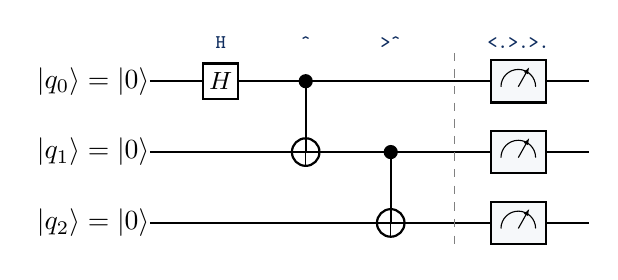
\begin{tikzpicture}[x=0.9cm, y=0.9cm, thick]
    % Wire labels
    \node at (-0.8, 2) {$\ket{q_0} = \ket{0}$};
    \node at (-0.8, 1) {$\ket{q_1} = \ket{0}$};
    \node at (-0.8, 0) {$\ket{q_2} = \ket{0}$};
    
    % Wires
    \draw (0, 2) -- (6.2, 2);
    \draw (0, 1) -- (6.2, 1);
    \draw (0, 0) -- (6.2, 0);
    
    % H on q0
    \node[above=8pt, font=\scriptsize\ttfamily, text=darkblue] at (1.0, 2) {H};
    \node[gate] at (1.0, 2) {$H$};
    
    % CNOT 0->1
    \node[above=8pt, font=\scriptsize\ttfamily, text=darkblue] at (2.2, 2) {\^{}};
    \node[control] at (2.2, 2) {};
    \draw[thick] (2.2, 2) -- (2.2, 1);
    \node[target] at (2.2, 1) {};
    
    % CNOT 1->2
    \node[above=8pt, font=\scriptsize\ttfamily, text=darkblue] at (3.4, 2) {>\^{}};
    \node[control] at (3.4, 1) {};
    \draw[thick] (3.4, 1) -- (3.4, 0);
    \node[target] at (3.4, 0) {};
    
    % Dashed separator
    \draw[dashed, thin, gray] (4.3, 2.4) -- (4.3, -0.4);
    
    % Measurements
    \node[above=8pt, font=\scriptsize\ttfamily, text=darkblue] at (5.2, 2) {<.>.>.};
    \node[bigmeter] at (5.2, 2) {};
    \node[bigmeter] at (5.2, 1) {};
    \node[bigmeter] at (5.2, 0) {};
\end{tikzpicture}%
}
\caption{Compiled circuit for $\ket{\text{GHZ}_3}$ preparation (\texttt{H\^{}>\^{}<.>.>.}).}
\end{figure}

\subsection{Quantum Teleportation Protocol}
Quantum teleportation \cite{bennett1993teleportation} transfers an arbitrary state $\ket{\psi} = \alpha\ket{0} + \beta\ket{1}$ from sender qubit $q_0$ to receiver qubit $q_2$ using an entangled Bell pair shared across $(q_1, q_2)$ and two classical feed-forward bits:

\begin{lstlisting}[caption={Quantum Teleportation in \texttt{|BF>}.}]
>H^<^H.>. [>+<+] < [>>Z<<+] >>
\end{lstlisting}

\begin{enumerate}
    \item \textbf{Bell Resource (\texttt{>H\^{}}):} Shifts pointer to $q_1$ and entangles $(q_1, q_2)$ into $\ket{\Phi^+}_{12} = \frac{1}{\sqrt{2}}(\ket{00} + \ket{11})$. The joint 3-qubit state factors into the Bell basis on $(q_0, q_1)$:
    \begin{equation}
    \begin{aligned}
        \ket{\Psi} = \frac{1}{2} \Big[ &\ket{\Phi^+}_{01} \ket{\psi}_2 + \ket{\Phi^-}_{01} (Z\ket{\psi})_2 \\
        + &\ket{\Psi^+}_{01} (X\ket{\psi})_2 + \ket{\Psi^-}_{01} (XZ\ket{\psi})_2 \Big]
    \end{aligned}
    \end{equation}
    \item \textbf{Bell Measurement (\texttt{<\^{}H.>.}):} Returns to $q_0$ via \texttt{<}, applies $\text{CNOT}_{0\to 1}$ (\texttt{\^{}}) and $H$ on $q_0$, and measures $q_0 \to c_0$ (\texttt{.}). Shifts to $q_1$ via \texttt{>} and measures $q_1 \to c_1$ (\texttt{.}). The pointer remains at cell $p = 1$.
    \item \textbf{Dynamic Feed-Forward (\texttt{[>+<+]<[>>Z<<+]>>}):} At $p = 1$, if $c_1 = 1$, the loop \texttt{[>+<+]} steps to $q_2$ (\texttt{>}), applies Pauli-$X$ (\texttt{+}), returns to $q_1$ (\texttt{<}), and flips $q_1$ from $\ket{1}$ to $\ket{0}$ via \texttt{+} (or reset \texttt{,}) to cleanly exit the dynamic while-loop after a single execution. Next, \texttt{<} moves the tape head to $q_0$; if $c_0 = 1$, \texttt{[>>Z<<+]} branches to $q_2$ (\texttt{>>}), applies Pauli-$Z$ (\texttt{Z}), returns to $q_0$ (\texttt{<<}), and flips $q_0$ to $\ket{0}$. Finally, \texttt{>>} parks the pointer at $q_2$, holding $\ket{\psi}$.
\end{enumerate}

\begin{figure}[h!]
\centering
\resizebox{0.96\columnwidth}{!}{%
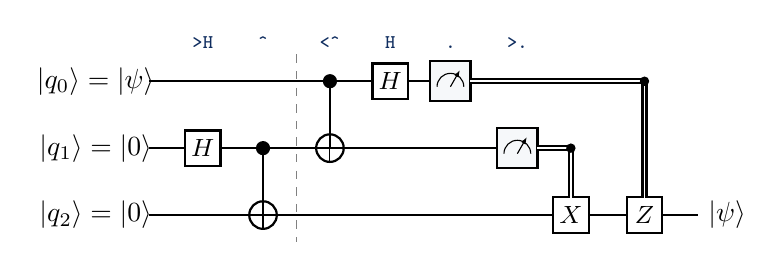
\begin{tikzpicture}[x=0.85cm, y=0.85cm, thick]
    % Wire labels
    \node at (-0.8, 2) {$\ket{q_0} = \ket{\psi}$};
    \node at (-0.8, 1) {$\ket{q_1} = \ket{0}$};
    \node at (-0.8, 0) {$\ket{q_2} = \ket{0}$};
    
    % Wires
    \draw (0, 2) -- (4.8, 2);
    \draw (0, 1) -- (5.8, 1);
    \draw (0, 0) -- (8.2, 0);
    \node[right] at (8.2, 0) {$\ket{\psi}$};
    
    % EPR: H on q1, CNOT 1->2
    \node[above=8pt, font=\scriptsize\ttfamily, text=darkblue] at (0.8, 2) {>H};
    \node[gate] at (0.8, 1) {$H$};
    
    \node[above=8pt, font=\scriptsize\ttfamily, text=darkblue] at (1.7, 2) {\^{}};
    \node[control] at (1.7, 1) {};
    \draw[thick] (1.7, 1) -- (1.7, 0);
    \node[target] at (1.7, 0) {};
    
    % Dashed separator
    \draw[dashed, thin, gray] (2.2, 2.4) -- (2.2, -0.4);
    
    % BSM: CNOT 0->1, H on q0
    \node[above=8pt, font=\scriptsize\ttfamily, text=darkblue] at (2.7, 2) {<\^{}};
    \node[control] at (2.7, 2) {};
    \draw[thick] (2.7, 2) -- (2.7, 1);
    \node[target] at (2.7, 1) {};
    
    \node[above=8pt, font=\scriptsize\ttfamily, text=darkblue] at (3.6, 2) {H};
    \node[gate] at (3.6, 2) {$H$};
    
    % Measurements
    \node[above=8pt, font=\scriptsize\ttfamily, text=darkblue] at (4.5, 2) {.};
    \node[meter, minimum size=0.51cm] (m0) at (4.5, 2) {};
    
    \node[above=8pt, font=\scriptsize\ttfamily, text=darkblue] at (5.5, 2) {>.};
    \node[meter, minimum size=0.51cm] (m1) at (5.5, 1) {};
    
    % Gates on q2
    \node[gate] (X) at (6.3, 0) {$X$};
    \node[gate] (Z) at (7.4, 0) {$Z$};
    
    % Classical feedforward
    \draw[double] (5.8, 1) -- (6.3, 1) -- (6.3, 0.255);
    \node[circle, fill=black, inner sep=0pt, minimum size=3.4pt] at (6.3, 1) {};
    
    \draw[double] (4.8, 2) -- (7.4, 2) -- (7.4, 0.255);
    \node[circle, fill=black, inner sep=0pt, minimum size=3.4pt] at (7.4, 2) {};
\end{tikzpicture}%
}
\caption{Quantum Teleportation circuit generated from \texttt{|BF>}.}
\end{figure}

\subsection{2-Qubit Grover Search Algorithm}
Grover's search \cite{grover1996fast} amplifies the amplitude of a marked state $\ket{\omega} \in \{0,1\}^2$ (here $\ket{\omega} = \ket{11}$) in a 4-element database using a single oracle query ($P(\ket{11}) = 1$). Because $\text{CZ}_{0,1} = (I \otimes H) \, \text{CNOT}_{0\to 1} \, (I \otimes H)$, a Controlled-$Z$ phase oracle is expressed in \texttt{|BF>} via the 7-token macro \texttt{>H<\^{}>H<} (three gates):

\begin{lstlisting}[caption={Complete 2-Qubit Grover search for $\ket{\omega} = \ket{11}$ in \texttt{|BF>}.}]
H>H< >H<^>H< H+>H+< >H<^>H< +H>+H< .>.
\end{lstlisting}

\begin{itemize}
    \item \textbf{Initialization (\texttt{H>H<}):} Prepares the uniform superposition $\ket{s} = H^{\otimes 2}\ket{00} = \frac{1}{2}(\ket{00} + \ket{01} + \ket{10} + \ket{11})$.
    \item \textbf{Phase Oracle $U_\omega$ (\texttt{>H<\^{}>H<}):} Applies $\text{CZ}_{0,1}$, flipping the phase of $\ket{11}$ to yield $\frac{1}{2}(\ket{00} + \ket{01} + \ket{10} - \ket{11})$.
    \item \textbf{Grover Diffuser $D = 2\ket{s}\bra{s} - I$ (\texttt{H+>H+< >H<\^{}>H< +H>+H<}):} Conjugates $\text{CZ}_{0,1}$ by $H^{\otimes 2} X^{\otimes 2}$, which yields $H^{\otimes 2}(I - 2\ketbra{00}{00})H^{\otimes 2} = -D$, i.e.\ the diffuser up to an irrelevant global phase, reflecting amplitudes about the mean to isolate $\ket{11}$ with probability 1.0.
\end{itemize}

\begin{figure}[h!]
\centering
\resizebox{0.96\columnwidth}{!}{%
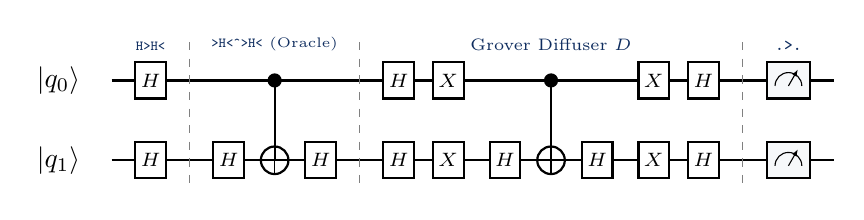
\begin{tikzpicture}[x=0.45cm, y=1.014cm, thick]
    % Wire labels
    \node at (-1.5, 1) {$\ket{q_0}$};
    \node at (-1.5, 0) {$\ket{q_1}$};
    
    % Wires
    \draw (0, 1) -- (20.4, 1);
    \draw (0, 0) -- (20.4, 0);
    
    % Stage 1: H>H<
    \node[above=7pt, font=\fontsize{5.5}{6.5}\selectfont\ttfamily, text=darkblue] at (1.1, 1) {H>H<};
    \node[smallgate] at (1.1, 1) {$H$};
    \node[smallgate] at (1.1, 0) {$H$};
    
    \draw[dashed, thin, gray] (2.2, 1.48) -- (2.2, -0.39);
    
    % Stage 2: Oracle
    \node[above=7pt, font=\fontsize{5.5}{6.5}\selectfont, text=darkblue] at (4.6, 1) {\texttt{>H<\^{}>H<} (Oracle)};
    \node[smallgate] at (3.3, 0) {$H$};
    \node[control] at (4.6, 1) {};
    \draw[thick] (4.6, 1) -- (4.6, 0);
    \node[target] at (4.6, 0) {};
    \node[smallgate] at (5.9, 0) {$H$};
    
    \draw[dashed, thin, gray] (7.0, 1.48) -- (7.0, -0.39);
    
    % Stage 3: Diffuser
    \node[above=7pt, font=\fontsize{6}{7}\selectfont, text=darkblue] at (12.4, 1) {Grover Diffuser $D$};
    \node[smallgate] at (8.1, 1) {$H$};
    \node[smallgate] at (9.5, 1) {$X$};
    \node[smallgate] at (8.1, 0) {$H$};
    \node[smallgate] at (9.5, 0) {$X$};
    
    \node[smallgate] at (11.1, 0) {$H$};
    \node[control] at (12.4, 1) {};
    \draw[thick] (12.4, 1) -- (12.4, 0);
    \node[target] at (12.4, 0) {};
    \node[smallgate] at (13.7, 0) {$H$};
    
    \node[smallgate] at (15.3, 1) {$X$};
    \node[smallgate] at (16.7, 1) {$H$};
    \node[smallgate] at (15.3, 0) {$X$};
    \node[smallgate] at (16.7, 0) {$H$};
    
    \draw[dashed, thin, gray] (17.8, 1.48) -- (17.8, -0.39);
    
    % Stage 4: Measurements
    \node[above=7pt, font=\fontsize{6}{7}\selectfont\ttfamily, text=darkblue] at (19.1, 1) {.>.};
    \node[meter] at (19.1, 1) {};
    \node[meter] at (19.1, 0) {};
\end{tikzpicture}%
}
\caption{2-Qubit Grover search circuit in \texttt{|BF>} isolating $\ket{11}$.}
\end{figure}

\section{Conclusion}
\texttt{|BF>} (Bra-Ket-Fuck) demonstrates that an esoteric quantum tape language need not sacrifice physical realism for mathematical minimalism. By grounding the Dirac--M\"uller Abstract Machine in the $\ket{0}^{\otimes N}$ ground state, adopting the universal Clifford+$T$ basis, and restricting the native two-qubit gate to nearest neighbors, \texttt{|BF>} can serve as a formal verification calculus, a compiler fuzzing target, and a compact front-end for OpenQASM 3.0 \cite{cross2022openqasm3}. Coherent (Profile C) control remains its main source of non-local, multi-qubit cost.

\begin{thebibliography}{99}

\bibitem{muller1993brainfuck}
U.~M{\"u}ller, ``Brainfuck,'' 1993, \href{https://en.wikipedia.org/wiki/Brainfuck}{online archive}.

\bibitem{bernstein1997quantum}
E.~Bernstein and U.~Vazirani, ``Quantum complexity theory,'' \emph{SIAM Journal on Computing}, vol.~26, no.~5, pp.~1411--1473, 1997, \href{https://doi.org/10.1137/S0097539796300921}{doi:10.1137/S0097539796300921}.

\bibitem{dirac1939notation}
P.~A.~M. Dirac, ``A new notation for quantum mechanics,'' \emph{Math. Proc. Cambridge Philos. Soc.}, vol.~35, no.~3, pp.~416--418, 1939, \href{https://doi.org/10.1017/S0305004100021162}{doi:10.1017/S0305004100021162}.

\bibitem{nielsen2010quantum}
M.~A. Nielsen and I.~L. Chuang, \emph{Quantum Computation and Quantum Information}, 10th Anniversary ed. Cambridge University Press, 2010, \href{https://doi.org/10.1017/CBO9780511976667}{doi:10.1017/CBO9780511976667}.

\bibitem{boykin1999optimal}
P.~O. Boykin, T.~Mor, M.~Pulver, V.~Roychowdhury, and F.~Vatan, ``A new universal and fault-tolerant quantum basis,'' \emph{Information Processing Letters}, vol.~75, no.~3, pp.~101--107, 2000, arXiv:\href{https://arxiv.org/abs/quant-ph/9906054}{quant-ph/9906054}.

\bibitem{bravyi2005universal}
S.~Bravyi and A.~Kitaev, ``Universal quantum computation with ideal Clifford gates and noisy ancillas,'' \emph{Phys. Rev. A}, vol.~71, no.~2, p.~022316, 2005, \href{https://doi.org/10.1103/PhysRevA.71.022316}{doi:10.1103/PhysRevA.71.022316}.

\bibitem{barenco1995elementary}
A.~Barenco, C.~H. Bennett, R.~Cleve, D.~P. DiVincenzo, N.~Margolus, P.~Shor, T.~Sleator, J.~A. Smolin, and H.~Weinfurter, ``Elementary gates for quantum computation,'' \emph{Phys. Rev. A}, vol.~52, no.~5, pp.~3457--3467, 1995, \href{https://doi.org/10.1103/PhysRevA.52.3457}{doi:10.1103/PhysRevA.52.3457}.

\bibitem{ozawa1998halting}
M.~Ozawa, ``Quantum nondemolition monitoring of universal quantum computers,'' \emph{Phys. Rev. Lett.}, vol.~80, no.~3, pp.~631--634, 1998, \href{https://doi.org/10.1103/PhysRevLett.80.631}{doi:10.1103/PhysRevLett.80.631}.

\bibitem{linden1998halting}
N.~Linden and S.~Popescu, ``The halting problem for quantum computers,'' 1998, arXiv:\href{https://arxiv.org/abs/quant-ph/9806054}{quant-ph/9806054}.

\bibitem{fowler2004lnn}
A.~G. Fowler, S.~J. Devitt, and L.~C.~L. Hollenberg, ``Implementation of Shor's algorithm on a linear nearest neighbour qubit array,'' \emph{Quantum Info. Comput.}, vol.~4, no.~4, pp.~237--251, 2004, arXiv:\href{https://arxiv.org/abs/quant-ph/0402196}{quant-ph/0402196}.

\bibitem{saeedi2011lnn}
M.~Saeedi, R.~Wille, and R.~Drechsler, ``Synthesis of quantum circuits for linear nearest neighbor architectures,'' \emph{Quantum Information Processing}, vol.~10, no.~3, pp.~355--377, 2011, \href{https://doi.org/10.1007/s11128-010-0201-2}{doi:10.1007/s11128-010-0201-2}.

\bibitem{ihope2006qbf}
Ihope127, ``Quantum brainfuck,'' \emph{Esolang: The Esoteric Programming Languages Wiki}, 2006, \href{https://esolangs.org/wiki/Quantum_brainfuck}{https://esolangs.org/wiki/Quantum\_brainfuck}.

\bibitem{cross2022openqasm3}
A.~W. Cross, A.~Javadi-Abhari, T.~Alexander, N.~de~Beaudrap, L.~S. Bishop, S.~Heidel, C.~A. Ryan, P.~Sivarajah, J.~Smolin, J.~M. Gambetta, and B.~R. Johnson, ``OpenQASM 3: A broader and deeper quantum assembly language,'' \emph{ACM Trans. Quantum Comput.}, vol.~3, no.~3, art.~12, pp.~1--50, 2022, \href{https://doi.org/10.1145/3505636}{doi:10.1145/3505636}.

\bibitem{rand2018voqc}
K.~Hietala, R.~Rand, S.-H. Hung, X.~Wu, and M.~Hicks, ``A verified optimizer for quantum circuits,'' \emph{Proc. ACM Program. Lang.}, vol.~5, no.~POPL, art.~37, 2021, \href{https://doi.org/10.1145/3434318}{doi:10.1145/3434318}.

\bibitem{preskill2018nisq}
J.~Preskill, ``Quantum Computing in the NISQ era and beyond,'' \emph{Quantum}, vol.~2, p.~79, 2018, \href{https://doi.org/10.22331/q-2018-08-06-79}{doi:10.22331/q-2018-08-06-79}.

\bibitem{arute2019supremacy}
F.~Arute, K.~Arya, R.~Babbush, et~al., ``Quantum supremacy using a programmable superconducting processor,'' \emph{Nature}, vol.~574, no.~7779, pp.~505--510, 2019, \href{https://doi.org/10.1038/s41586-019-1666-5}{doi:10.1038/s41586-019-1666-5}.

\bibitem{greenberger1989ghz}
D.~M. Greenberger, M.~A. Horne, and A.~Zeilinger, ``Going beyond Bell's Theorem,'' in \emph{Bell's Theorem, Quantum Theory and Conceptions of the Universe}, pp.~69--72, Kluwer Academic, 1989, arXiv:\href{https://arxiv.org/abs/0712.0921}{0712.0921}.

\bibitem{bennett1993teleportation}
C.~H. Bennett, G.~Brassard, C.~Cr{\'e}peau, R.~Jozsa, A.~Peres, and W.~K. Wootters, ``Teleporting an unknown quantum state via dual classical and Einstein-Podolsky-Rosen channels,'' \emph{Phys. Rev. Lett.}, vol.~70, no.~13, pp.~1895--1899, 1993, \href{https://doi.org/10.1103/PhysRevLett.70.1895}{doi:10.1103/PhysRevLett.70.1895}.

\bibitem{grover1996fast}
L.~K. Grover, ``A fast quantum mechanical algorithm for database search,'' in \emph{Proc. 28th Ann. ACM Symp. Theory of Computing (STOC '96)}, pp.~212--219, 1996, \href{https://doi.org/10.1145/237814.237866}{doi:10.1145/237814.237866}.

\end{thebibliography}

\end{document}
